\section{Method}
\label{sec:method}

To navigate complex, dynamic human environments, a robot must do more than treat sound as a geometric goal. SAVNav processes social sound events as persistent social boundaries. The system operates through a three-stage pipeline, as illustrated in Fig.~\ref{fig:system_arch}: First, multi-modal perception extracts persistent human and acoustic entities from the visual and auditory streams. Second, SAVMap fuses these entities into target locations and spatial social boundaries. Finally, the SAVNav policy acts on SAVMap: if the acoustic target remains unanchored, it seeks an optimal viewpoint for active sensory exploration; given an anchored target or a selected viewpoint, it generates a socially-compliant navigation path that explicitly yields to the modeled boundaries.

\begin{figure*}[t]
    \centering
    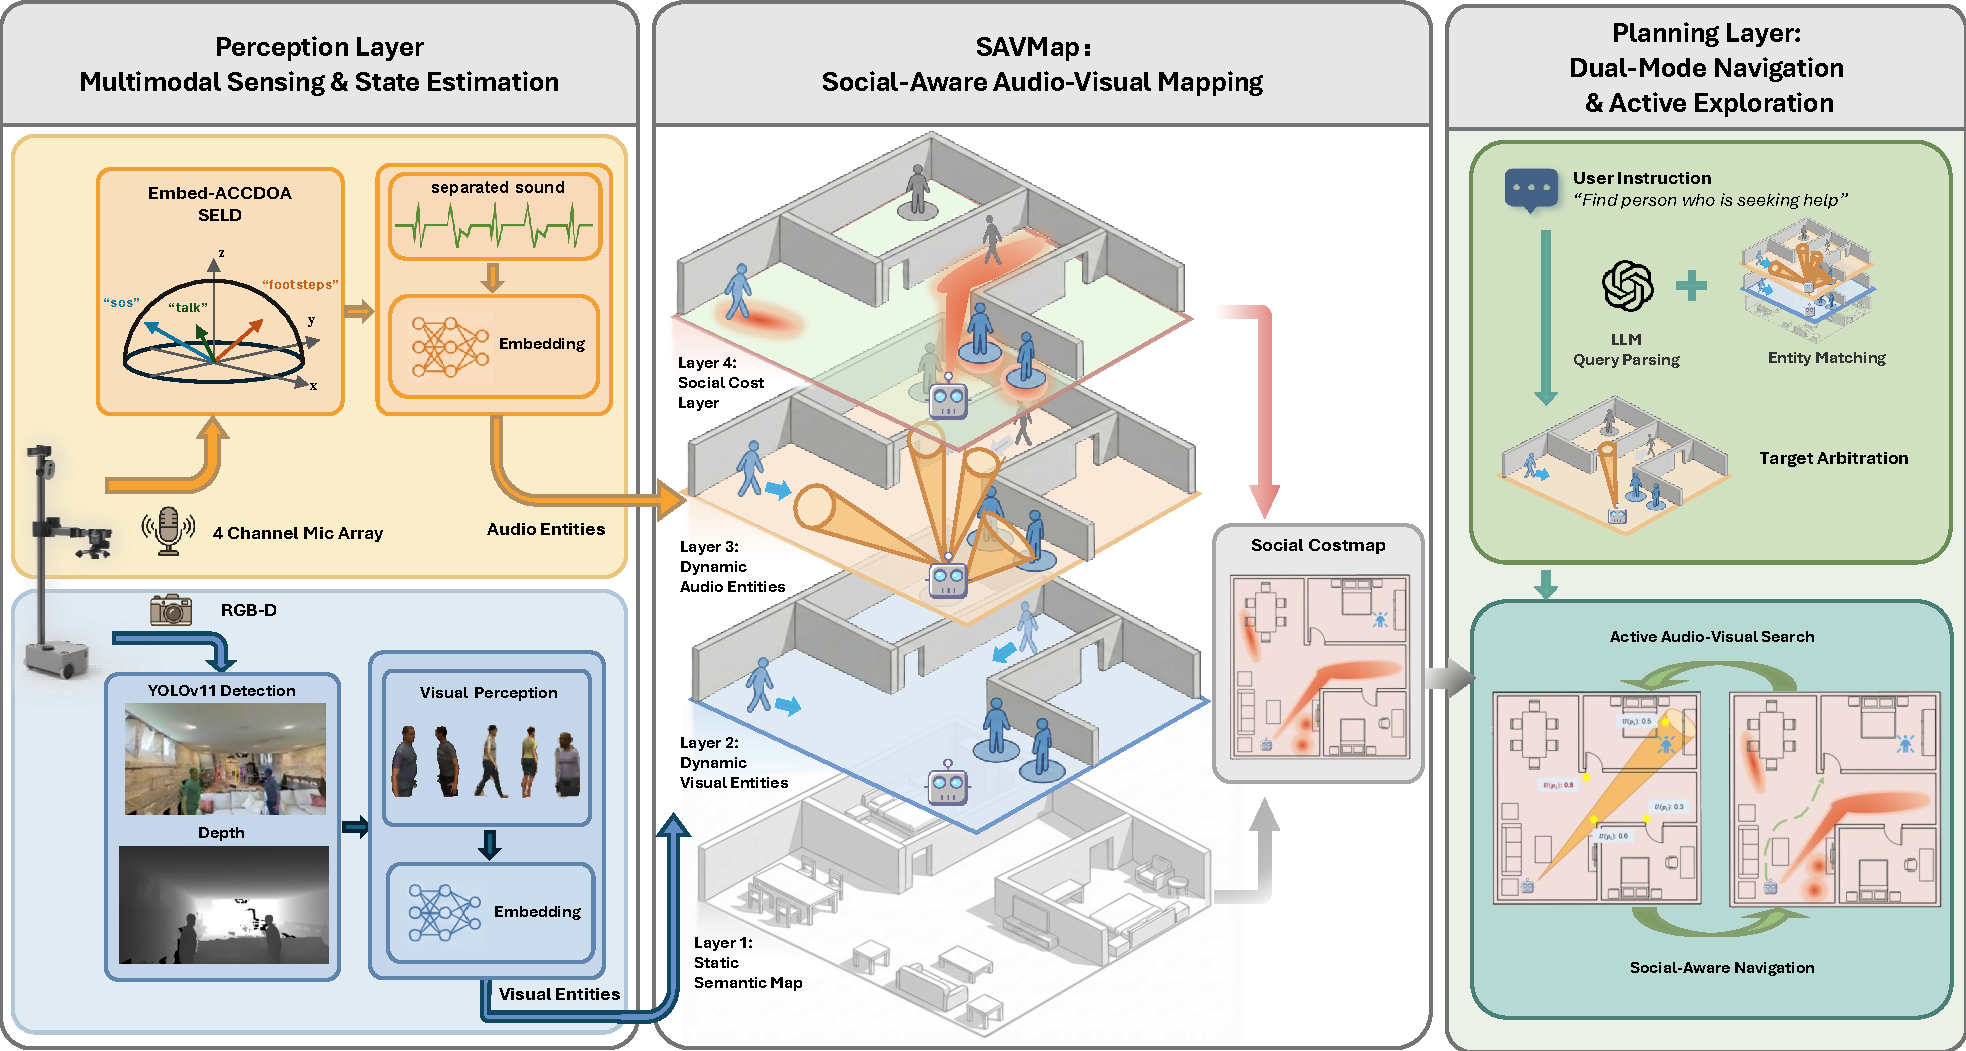
\includegraphics[width=1.00\linewidth]{figures/method.pdf}
    \caption{System architecture of SAVNav. The framework operates through a three-stage pipeline. First, multi-modal perception extracts spatial and semantic attributes of both sound events and visual human entities. Second, acoustic-to-spatial social mapping (SAVMap) projects these entities into a layered representation to construct a social cost field, explicitly modeling both line-of-sight humans and topology-aware non-line-of-sight acoustic risks. Finally, the SAVNav policy either executes active sensory exploration to resolve unanchored acoustic targets or generates a socially-compliant reference path using the Fast Marching Method (FMM).}
    \label{fig:system_arch}
\end{figure*}

\subsection{Problem Formulation and Notation}
\label{subsec:problem_formulation}

We formalize the SAVNav task in a continuous 3D environment $\mathcal{W}$, comprising physical obstacles and dynamic human actors $\mathcal{H} = \{h_1, \dots, h_N\}$. The environment generates sound events $\mathcal{A}$ belonging to two semantic classes: target sound events with labels $\mathcal{L}_{\mathrm{target}} = \{$\texttt{doorbell}, \texttt{human call}, \texttt{television}, \texttt{water tap}$\}$ and social sound events with labels $\mathcal{L}_{\mathrm{social}} = \{$\texttt{footsteps}, \texttt{conversation}$\}$. The robot is provided with a static semantic map containing a 2D navigable grid $\mathcal{M}_{\mathrm{nav}}$, an obstacle distance field $\mathcal{D}_{\mathrm{obs}}$, precomputed topological nodes $\mathcal{N}_{\mathrm{topo}}$, and a set of static objects $\mathcal{O}$. Each static object $o \in \mathcal{O}$ is annotated with its 3D spatial coordinates, oriented bounding box, and a pre-computed ImageBind~\cite{ImageBindOneEmbedding2023} cross-modal embedding $\mathbf{e}_{\mathrm{obj}}$. While this map is known, the robot does not observe the ground-truth states of $\mathcal{H}$, and must dynamically perceive the events from $\mathcal{A}$ corresponding to $\mathcal{L}_{\mathrm{social}}$ emitted by these actors to infer unobservable social boundaries.

Each episode specifies a query $q \in \mathcal{L}_{\mathrm{target}}$ identifying the navigation goal. At each time step $t$, the robot state is denoted by its $\mathrm{SE}(3)$ pose, from which we extract its 3D position $\mathbf{p}_{\mathrm{robot}}^{(t)} \in \mathbb{R}^3$. The robot receives a multimodal observation $O^{(t)} = (I^{(t)}, D^{(t)}, A^{(t)})$ consisting of an RGB image $I^{(t)}$, an aligned depth map $D^{(t)}$, and an acoustic waveform $A^{(t)}$. The objective is to compute velocity commands $\mathbf{v}^{(t)}$ to reach a state where $\|\mathbf{p}_{\mathrm{robot}}^{(t)} - \mathbf{p}_{\mathrm{target}}\| \le d_{\mathrm{success}}$ within the maximum allowable time steps $T$ while explicitly avoiding collisions with any human actor, where $\mathbf{p}_{\mathrm{target}}$ is the target's ground-truth location and $d_{\mathrm{success}}$ is the distance threshold. Table~\ref{tab:notation} summarizes the main notation used below.

\begin{table}[ht]
    \centering
    \caption{Summary of key notations}
    \label{tab:notation}
    \resizebox{\linewidth}{!}{
        \begin{tabular}{cl}
            \toprule
            \textbf{Symbol}                                                & \textbf{Definition}                                                             \\
            \midrule
            $\mathcal{L}_{\mathrm{target}}, \mathcal{L}_{\mathrm{social}}$ & Semantic label sets for target and social sound events                          \\
            $\mathbf{p}_{\mathrm{hum}}, \sigma_{\mathrm{hum}}$             & 3D position and spatial uncertainty of a visually detected human                \\
            $\mathbf{d}_{\mathrm{aud}}, \sigma_{\mathrm{aud}}$             & World-frame acoustic DOA vector and its angular uncertainty                     \\
            $B_{\mathrm{anch}}^{(t)}(E_{\mathrm{vis}})$                    & Anchoring confidence linking a sound event to visual entity $E_{\mathrm{vis}}$ \\
            $B_{\mathrm{nlos}}^{(t)}(n_j)$                                 & Topology-aware NLOS risk inferred at candidate node $n_j$                       \\
            $C_{\mathrm{social}}(\mathbf{x})$                              & Continuous social cost field evaluated at spatial location $\mathbf{x}$         \\
            $B^{(t)}(\mathbf{x})$                                          & Target belief map (log-odds evidence grid)                              \\
            $U^{(t)}(\mathbf{p}_i)$                                        & Utility of sampling candidate viewpoint $\mathbf{p}_i$                          \\
            $F(\mathbf{x})$                                                & Speed field used in the Fast Marching Method (FMM) planner                      \\
            \bottomrule
        \end{tabular}
    }
\end{table}

\subsection{Multi-Modal Perception}
\label{subsec:perception}

As depicted in the left panel of Fig.~\ref{fig:system_arch}, the perception layer extracts spatial and semantic attributes from raw sensory streams and transforms them into object-centric representations.

\subsubsection{Visual Perception}
The visual module processes egocentric RGB-D observations using YOLO26~\cite{YOLO26KeyArchitectural2026} for real-time human detection and segmentation. For each detected human mask, we extract its 3D position $\mathbf{p}_{\mathrm{hum}} \in \mathbb{R}^3$ via depth projection and assign a spatial uncertainty $\sigma_{\mathrm{hum}}$ that scales quadratically with distance. We crop the masked region and encode it with ImageBind~\cite{ImageBindOneEmbedding2023} to obtain a cross-modal embedding $\mathbf{e}_{\mathrm{hum}}$. To maintain temporal consistency, these frame-level detections are continuously tracked, with each managed as a persistent human entity $E_{\mathrm{hum}} = (\mathbf{p}_{\mathrm{hum}}, \sigma_{\mathrm{hum}}, \mathbf{e}_{\mathrm{hum}})$. For static objects $\mathcal{O}$, their spatial attributes and embeddings $\mathbf{e}_{\mathrm{obj}}$ are simply retrieved from the static semantic map.

\subsubsection{Acoustic Perception}
The acoustic module processes continuous first-order Ambisonics (FOA) audio streams using a sliding-window strategy. Audio clips are fed into embed-ACCDOA~\cite{OpenvocabularySoundEvent2025} to extract a set of concurrent sound events, each yielding an egocentric direction-of-arrival (DOA) and a CLAP embedding~\cite{CLAPLearningAudio2023}. For each detected event, by comparing its embedding against the text CLAP embeddings of expected labels ($\{q\} \cup \mathcal{L}_{\mathrm{social}}$), we classify the sound and encode its text class label $c_{\mathrm{aud}}$ with ImageBind to obtain an acoustic embedding $\mathbf{e}_{\mathrm{aud}}$. The egocentric DOA is transformed into a world-frame directional vector $\mathbf{d}_{\mathrm{aud}}^{(t)} \in \mathbb{R}^3$, and we assign an angular uncertainty $\sigma_{\mathrm{aud}}$ scaled by the embed-ACCDOA model confidence. Since embed-ACCDOA outputs stateless detections for multiple simultaneous sounds, the module temporally associates these signals across windows using spatial DOA proximity and ImageBind cosine similarity to maintain a set of persistent sound events, where each event is denoted as $E_{\mathrm{aud}} = (\mathbf{d}_{\mathrm{aud}}, \sigma_{\mathrm{aud}}, \mathbf{e}_{\mathrm{aud}}, c_{\mathrm{aud}})$.

\subsection{Acoustic-to-Spatial Social Mapping (SAVMap)}
\label{subsec:savmap}

Vision-based social navigation relies on LOS detections. SAVMap maintains three coupled states: anchoring confidence for audio-visual association, NLOS risk belief over topological nodes, and the resultant social cost field used by the SAVNav policy.

\subsubsection{Audio-Visual Anchoring}
The association between a persistent sound event $E_{\mathrm{aud}}$ and a visual entity $E_{\mathrm{vis}}$ (either a tracked LOS human entity $E_{\mathrm{hum}}$ or a static object $o$, depending on $c_{\mathrm{aud}}$) is governed by a first-order Markov smoothing update. The anchoring confidence combines semantic cross-modal similarity $s$ with a Gaussian penalty on angular spatial deviation:
\begin{equation}
    B_{\mathrm{anch}}^{(t)}(E_{\mathrm{vis}}) = \lambda_{\mathrm{anch}} B_{\mathrm{anch}}^{(t-1)}(E_{\mathrm{vis}}) + \eta_{\mathrm{anch}} \cdot s \cdot \exp\left(-\frac{\Delta\theta_\mathrm{vis}^{(t)2}}{2\sigma_{\mathrm{aud}}^2}\right),
    \label{eq:anch_update}
\end{equation}
where $s \in [-1, 1]$ is the cosine similarity between the acoustic embedding $\mathbf{e}_{\mathrm{aud}}$ and the visual entity's ImageBind embedding $\mathbf{e}_{\mathrm{vis}}$ (i.e., $\mathbf{e}_{\mathrm{hum}}$ or $\mathbf{e}_{\mathrm{obj}}$), \allowbreak$\Delta\theta_\mathrm{vis}^{(t)}$ is the angular deviation in radians between the visual entity's spatial direction relative to the robot and the acoustic DOA $\mathbf{d}_{\mathrm{aud}}^{(t)}$, and $\lambda_{\mathrm{anch}}, \eta_{\mathrm{anch}}$ are the decay and innovation rates, respectively. Values are strictly clamped to $[0,1]$. If the sound event is not detected or the entity lies far outside the angular bounds defined by $\sigma_{\mathrm{aud}}$, the innovation term becomes negligible, yielding exponential decay via $\lambda_{\mathrm{anch}}$. The visual entity with the highest confidence exceeding an engagement threshold $\tau_{\mathrm{anch}}$ is selected as the anchored source, inheriting its 3D position and spatial uncertainty.

\subsubsection{Topology-Aware Acoustic Anticipation}
When an event $E_{\mathrm{aud}}$ with a label in $\mathcal{L}_{\mathrm{social}}$ remains unanchored to any LOS visual entity, SAVMap infers NLOS risk over the precomputed topological nodes $\mathcal{N}_{\mathrm{topo}}$. Analogous to the visual anchoring dynamics, the risk belief for each topological node $n_j$ is updated based on its spatial alignment with the acoustic DOA:
\begin{equation}
    B_{\mathrm{nlos}}^{(t)}(n_j) = \lambda_{\mathrm{nlos}} B_{\mathrm{nlos}}^{(t-1)}(n_j) + \eta_{\mathrm{nlos}} \exp\left(-\frac{\Delta\theta_j^{(t)2}}{2\sigma_{\mathrm{aud}}^2}\right),
    \label{eq:nlos_score}
\end{equation}
where $\Delta\theta_j^{(t)} = \phi(\mathbf{p}_{n_j} - \mathbf{p}_{\mathrm{robot}}^{(t)}, \allowbreak \mathbf{d}_{\mathrm{aud}}^{(t)})$ is the angular deviation in radians. Values are strictly clamped to $[0,1]$. Nodes falling far outside the angular bounds of $\sigma_{\mathrm{aud}}$ naturally undergo exponential decay via $\lambda_{\mathrm{nlos}}$ due to the negligible exponential term. This risk representation is tied to the unanchored state: if $E_{\mathrm{aud}}$ ceases or successfully anchors to a visual entity, the associated NLOS scores are cleared, transferring the boundary from inferred topology to the observed entity.

We extract the most probable emergence node $n^* = \arg\max_{n_j} B_{\mathrm{nlos}}^{(t)}(n_j)$. If $B_{\mathrm{nlos}}^{(t)}(n^*) > \tau_{\mathrm{nlos}}$ and $c_{\mathrm{aud}} = \texttt{footsteps}$, the robot assigns a conservative velocity hypothesis pointing directly toward itself:
\begin{equation}
    \mathbf{v}_{*}^{(t)} = v_{\mathrm{walk}} \cdot \frac{\mathbf{p}_{\mathrm{robot}}^{(t)} - \mathbf{p}_{n^*}}{\|\mathbf{p}_{\mathrm{robot}}^{(t)} - \mathbf{p}_{n^*}\|},
    \label{eq:vel_hyp}
\end{equation}
where $v_{\mathrm{walk}}$ is a reference walking speed. For \texttt{conversation}, $n^*$ is treated as a stationary social boundary.

\subsubsection{Social Cost Fields}
SAVMap translates both visually confirmed LOS entities and inferred NLOS risks into spatial cost distributions.

The NLOS cost field $C_{\mathrm{nlos}}(\mathbf{x})$ is generated at the dominant topological node $n^*$. For stationary \texttt{conversation}, it follows an isotropic Gaussian:
\begin{equation}
    C_{\mathrm{nlos}}(\mathbf{x}) = B_{\mathrm{nlos}}^{(t)}(n^*) \cdot A \exp\left(-\frac{\|\mathbf{x} - \mathbf{p}_{n^*}\|^2}{2\sigma^2_{\mathrm{scg}}}\right),
    \label{eq:scg_cost}
\end{equation}
where $A$ is the base amplitude and $\sigma_{\mathrm{scg}}$ defines the spatial radius. For \texttt{footsteps}, it takes an anisotropic form extending along the velocity hypothesis $\mathbf{v}_{*}^{(t)}$:
\begin{equation}
    C_{\mathrm{nlos}}(\mathbf{x}) = B_{\mathrm{nlos}}^{(t)}(n^*) \cdot A \exp \left( - \frac{x_*^2}{2\sigma_{x,*}^2} - \frac{y_*^2}{2\sigma_y^2} \right),
    \label{eq:dp_cost}
\end{equation}
where $x_*$ and $y_*$ are the longitudinal and lateral projections of $\mathbf{x} - \mathbf{p}_{n^*}$ onto $\mathbf{v}_{*}^{(t)}$. The forward spread $\sigma_{x,*}$ scales proportionally with $\|\mathbf{v}_{*}^{(t)}\|$, while the lateral variance $\sigma_y$ remains constant.

For anchored entities, the LOS cost field $C_{\mathrm{los}}(\mathbf{x})$ evaluates identical Gaussian forms centered deterministically at the tracked visual position $\mathbf{p}_{\mathrm{hum}}$, utilizing the observed human velocity $\mathbf{v}_{\mathrm{hum}}$ rather than a hypothesis. The final continuous social cost field aggregates these constraints, strictly bounded to prevent cost explosion:
\begin{equation}
    C_{\mathrm{social}}(\mathbf{x}) = \min\left(1, C_{\mathrm{los}}(\mathbf{x}) + C_{\mathrm{nlos}}(\mathbf{x})\right).
    \label{eq:final_cost}
\end{equation}

\subsection{Proactive Socially-Aware Navigation Policy (SAVNav policy)}
\label{subsec:savnav}

The SAVNav policy translates SAVMap into safe, target-driven motion. It operates on two map-level representations: the target belief map for acoustic target search and the social cost field for social compliance.

\subsubsection{Active Sensory Exploration}
As outlined by the decision logic in Fig.~\ref{fig:system_arch} (top right), if the acoustic target is detected but remains unanchored due to occlusion or reverberation, the robot enters active sensory exploration. We maintain a target belief map $B^{(t)}(\mathbf{x})$ over the navigable space, which functions as an evidence grid storing log-odds probabilities of the target's presence. Following standard Bayesian mapping semantics, $B^{(t)}$ receives positive log-odds updates in the angular region aligned with the acoustic DOA $\mathbf{d}_{\mathrm{aud}}^{(t)}$ bounded by $\sigma_{\mathrm{aud}}$, and receives negative log-odds decay in any free space cleared by the robot's visual frustum.

To resolve target ambiguity, the robot samples candidate viewpoints $\mathcal{P} = \{\mathbf{p}_1, \dots, \mathbf{p}_K\}$ near topological nodes. The optimal viewpoint $\mathbf{p}^*$ is selected by maximizing the following utility:
\begin{equation}
    U^{(t)}(\mathbf{p}_i) = \sum_{\mathbf{c} \in \mathcal{S}(\mathbf{p}_i)} P_{\mathrm{target}}(\mathbf{c}) - \beta \frac{L(\mathbf{p}_{\mathrm{robot}}^{(t)}, \mathbf{p}_i)}{v_{\mathrm{avg}}},
    \label{eq:utility}
\end{equation}
where $\mathcal{S}(\mathbf{p}_i)$ defines the set of unoccluded discrete spatial grid cells visible from viewpoint $\mathbf{p}_i$, and $P_{\mathrm{target}}(\mathbf{c}) \in [0,1]$ is the target probability mapped from the log-odds grid $B^{(t)}$. $L(\cdot)$ is the geodesic path length from current position $\mathbf{p}_{\mathrm{robot}}^{(t)}$, $v_{\mathrm{avg}}$ is the nominal exploration speed, and $\beta$ balances information gain against travel time.

\subsubsection{Socially-Compliant Navigation}
As depicted in the bottom right panel of Fig.~\ref{fig:system_arch}, once the acoustic target is anchored or a viewpoint $\mathbf{p}^*$ is selected, the system projects the social cost field onto the 2D navigation grid $\mathcal{M}_{\mathrm{nav}}$ and computes global trajectories using the Fast Marching Method (FMM)~\cite{FastMarchingMethods1999} to solve the Eikonal equation. The scalar speed field driving the wave propagation is scaled inversely with the social cost:
\begin{equation}
    F(\mathbf{x}) = (F_{\max} - F_{\min}) \cdot \left(1 - C_{\mathrm{social}}(\mathbf{x})\right) + F_{\min},
    \label{eq:speed}
\end{equation}
where $F_{\max}$ and $F_{\min}$ are the robot's physical speed limit and the strictly positive minimum permissible speed. By smoothly diminishing the wave propagation speed across high-risk NLOS nodes and LOS humans, gradient descent over the resulting arrival-time landscape naturally yields reference paths that curve away from these social boundaries. These paths are then executed by the robot's local motion controller.
